\documentclass[a4paper,class=article,border=10pt,tikz]{standalone}
\usepackage{tikz}
\usetikzlibrary{snakes,calc,positioning,patterns,angles,quotes,decorations.pathmorphing,decorations.markings,through}
\usetikzlibrary{arrows,decorations,decorations.text}
\usepackage{rotating}
\usetikzlibrary{arrows,decorations,decorations.text}
\usetikzlibrary{patterns.meta,math}




\usepackage{siunitx}
\usepackage{pstricks}

\begin{document}

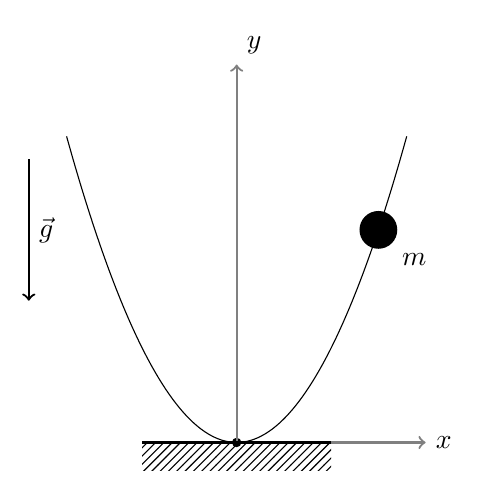
\begin{tikzpicture}[scale=1.2]
 \coordinate (origo) at (0,0);
 \coordinate (pivot) at (1,5);

 

    % draw axes
    \fill[black] (origo) circle (0.05);
    \draw[thick,gray,->] (origo) -- ++(2,0) node[black,right] {$x$};
    \draw[thick,gray,->] (origo) -- ++(0,4) node (mary) [black,above right] {$y$};
    \draw[thick,<-] (-2.2,1.5) -- (-2.2,3) node[midway, right] {$\vec{g}$};
    
    
    
    %\draw ($(origo)+(-2,4)$) parabola bend (origo) ($(origo)+(2,4)$) node[below right] {$a \cdot x^2$};
    \draw[black]   plot[smooth,domain=-1.8:0] (\x, {-\x^2}) node[below right] {};
    \draw[black]   plot[smooth,domain=0:1.8] (\x, {\x^2}) node[below right] {};

 

    % draw roof
    %\fill[pattern = north east lines] ($ (origo) + (-1,0) $) rectangle ($ (origo) + (1,0.3) $);
    \fill[pattern = north east lines] (-1,0) rectangle +(2,-0.3);
    \draw[thick] ($ (origo) + (-1,0) $) -- ($ (origo) + (1,0) $);

 

    %\node (bob1)  at ($(origo) +(2cm,4cm)$) [near end, right] {$m$};
    %\node (l1_label) at ($(origo)+(310:1.5cm)$)   {$l$};
    \fill (1.5, 2.25) circle (0.2) node[below right=0.25cm] {$m$};

 

    %\pic [draw, ->, "$\varphi_{1}$", angle eccentricity=1.9] {angle = mary--origo--bob1};

 

\end{tikzpicture}
\end{document}